\documentclass[25pt,margin=20mm,innermargin=-6in,blockverticalspace=1mm]{tikzposter}
\geometry{paperwidth=47in,paperheight=33in}
\usepackage[utf8]{inputenc}
\usepackage{amsmath}
\usepackage{amsfonts}
\usepackage{amsthm}
\usepackage{amssymb}
\usepackage{mathrsfs}
\usepackage{graphicx}
\usepackage{caption}
\usepackage{subcaption}
\usepackage{adjustbox}
\usepackage{enumitem}
\usepackage{wrapfig}
\usepackage{booktabs}
\usepackage{pifont}
\usepackage{array}
\usepackage[backend=bibtex,style=numeric,doi=false,url=false,eprint=false,sorting=none,autocite=superscript]{biblatex}
\usepackage{bodl}
\usetikzlibrary{positioning,shapes,arrows}

\makeatletter
\def\title#1{\gdef\@title{\scalebox{\TP@titletextscale}{%
\begin{minipage}[t]{\linewidth}
\centering
#1
\par
\vspace{0.5em}
\end{minipage}%
}}}
\makeatother


\addbibresource{bibliography.bib}
\AtBeginBibliography{\footnotesize}

% set theme parameters
\tikzposterlatexaffectionproofoff
\usetheme{UofATheme}
\usecolorstyle{UofAStyle}

\title{Using Alternate References for Transcriptome Analysis of an Indigenous Australian Study Cohort}
\author{\centering \textbf{Stevie Pederson}\textsuperscript{1,2},Yassine Souilmi\textsuperscript{1,3} Hardip Patel\textsuperscript{2}, Alex Brown\textsuperscript{1,2}, Jimmy Breen\textsuperscript{1,2}}
\institute{
  \textsuperscript{1}Black Ochre Data Labs, Telethon Kids Institute
  \textsuperscript{2}John Curtin School of Medical Research, Australian National University\\
  \textsuperscript{3}School of Biological Sciences, University of Adelaide
}


% begin document
\begin{document}
\maketitle

\node [below right=28mm and 8mm] at (bottomleft |- topright) {
\includegraphics[width=0.12\textwidth]{bodl_logo_white_background.jpg}};
\node [below left=20mm and 10mm] at (topright) {
\includegraphics[width=0.1\textwidth]{tki.jpg}};


\centering

%\block{Abstract}{
%Alignment of transcriptomic data to the standard reference genome has recently been shown to be a problematic strategy\autocite{Kaminow2022-dz}. 
%This is particularly relevant for populations which are poorly represented within existing repositories that capture global diversity, and when these populations themselves are known to contain a poorly characterised amount of unique variation.\\
%
%The use of an alternate reference genome which incorporates an appropriate set of variants has also been shown to improve alignments and quantifications at the gene level. 
%We propose that we will incorporate variant sets from public repositories as well as a custom set of variants identified within our study cohort and assess the impact on gene quantification across each alternate reference genome. 
%This is then extended into transcript-level quantification and the incorporation of user-defined sets of variants into an alternate reference transcriptome.
%In addition, a tool for creating custom reference transcriptomes has been developed.
%
%}

\begin{columns}
    \column{0.34}
    	\block{Genomic Variability}{
		\large
        \begin{minipage}{0.72\linewidth}
		The Indigenous Australian population contains a large amount of unique genetic diversity.       
				Given that risk factors are increasingly being shown to be polygenic and dependent on the genetic background. ignoring diversity in a large cohort may limit our ability to address this contribution. 
        \end{minipage}
        \hspace{5mm}
        \begin{minipage}{0.25\linewidth}
        \centering
        \small
        	
\includegraphics[scale=1]{25_unique.png} \\
        	Genomic variants unique to Indigenous Australians\autocite{Easteal2020-fo}
        \end{minipage}
        \vspace{1cm}
		
		The historical relationship between researchers and the Aboriginal community \textit{has been problematic	} and as such, this population is poorly represented in databases such as the 1000 Genomes Project (1000GP), and the Human Genome Diversity Project (HGDP).
%		Prepared in a highly consultative, and indigenous-led manner, the PROPHECY study present a unique opportunity to provide access to precision medicine for members of the Indigenous Australian community.
%		The unique design of the study also presents a unique opportunity to include population-level diversity across all -omics layers in the study.

    	}
    	\vspace{-1cm}
    	
    	\block{Variants from the 1000 Genomes Project}{
		\large
		
		Taking consensus 1000GP variants (>50\%) as a \textit{proof-of-principle}, a gene-level analysis (\textit{STARconsensus}\autocite{Kaminow2022-dz}) was prepared comparing the standard hg38 reference against a modified reference incorporating SNPs and InDels from the 1000GP.\\[5mm]

		\centering
		\begin{tabular}{p{11cm}rrrr}

		\toprule
		Region & SNV & Insertion & Deletion & \textbf{Total} \\ 
		  \midrule
		No Classified Region & 1,281,298 & 110,072 & 113,176 & \textbf{1,504,546} \\ 
		  Promoter & 151,537 & 13,775 & 14,616 & \textbf{179,928} \\ 
		  Upstream Promoter & 100,273 & 9,848 & 9,845 & \textbf{119,966 }\\ 
		  Exon & 68,628 & 4,682 & 4,814 & \textbf{78,124} \\ 
		  UTR & 24,213 & 2,197 & 2,261 & \textbf{28,671} \\ 
		  Splice Junction & 1,628 & 236 & 265 & \textbf{2,129 }\\ 
		  Stop Codon &  36 &   1 &   5 &  \textbf{42} \\ 
		  Start Codon &  16 &   3 &   2 &  \textbf{21} \\ 
		   \bottomrule
		\end{tabular}
		\vspace{1cm}
		
		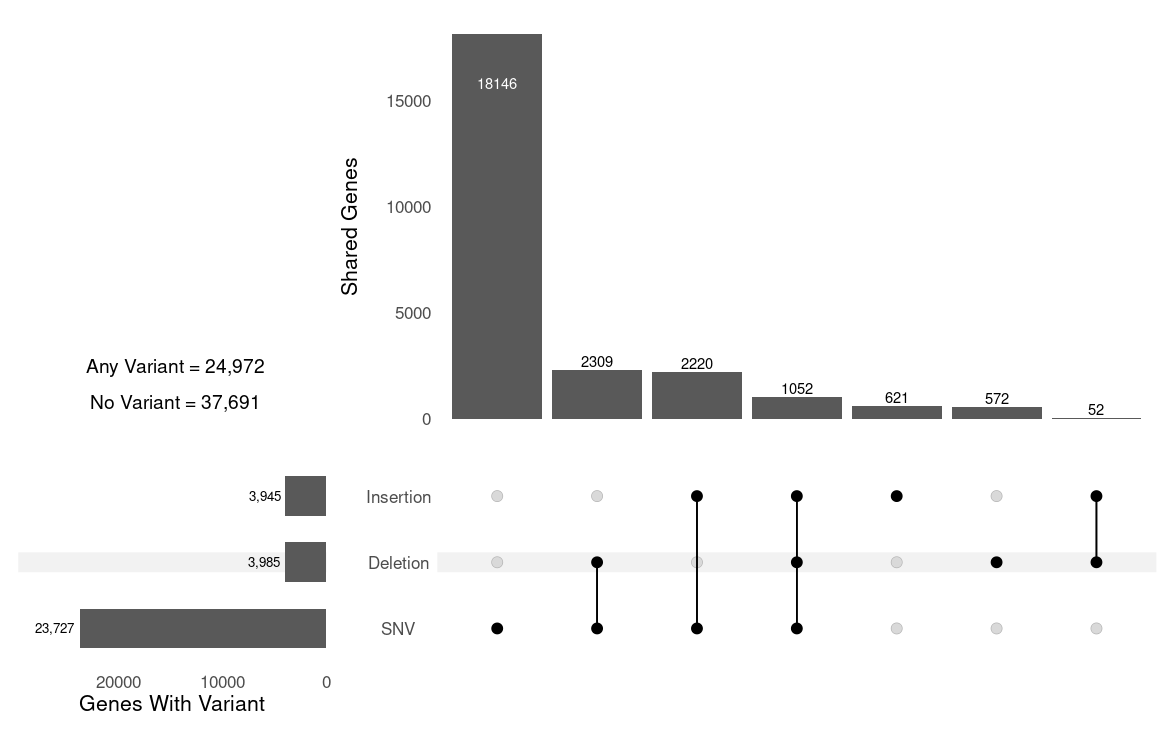
\includegraphics[scale=0.95]{var-in-genes.png} 
		~\\
		\normalsize
		\textit{Genes with variants overlapping an exon}



    	}
    	\vspace{-1cm}
    


    \column{0.34}
    \useblockstyle{KeyBlockStyle}
    \block{The PROPHECY Study}{
    \Large
    \vspace{2mm}
    The PROPHECY study (\textbf{P}reventing \textbf{R}enal, \textbf{OP}hthalmic and \textbf{H}eart \textbf{E}vents in \textbf{C}ommunit\textbf{Y}) consists of $\sim$1400 indigenous participants drawn from regional, remote and urban locations within South Australia.
    Amongst community, the study is colloquially known as the \textit{Aboriginal Diabetes Study}.\\
    
    The PROPHECY Study is a multi-omics study including genomic variants, DNA methylation, bulk RNA-Seq, proteomics, lipidomics, metabolomics and multiple other layers, all derived from blood samples taken from the same participants.
    
    \vspace{3mm}
    }
    \useblockstyle{UofABlockStyle}

    \block{Haploid Reference Strategies}{
    \Large
    Haploid reference strategies are well understood\, making these the first starting point for adressing issues of unique diversity.
    We are also exploring \textit{pan-genome, graph-based approaches\autocite{Sibbesen2023-md}}.\\[1cm]
    
    
    
    \begin{minipage}{\linewidth}
    \centering
    \begin{tabular}{p{14cm}>{\centering\arraybackslash}p{9cm}>{\centering\arraybackslash}p{9cm}}
    		\toprule
    		& \multicolumn{2}{c}{Reference Type} \\
    		\cline{2-3}
    		& Genome & Transcriptome \\
    		\midrule
    		Gene-Level Analysis & \textcolor{BodlGreen}{\ding{52}} & \textcolor{BodlGreen}{\ding{52}} \\
    		Transcript-Level Analysis\autocite{Baldoni2023-wm} & \textcolor{DarkRed}{\ding{54}} & \textcolor{BodlGreen}{\ding{52}} \\
    		Alignment Co-Ordinates & \textcolor{BodlGreen}{\ding{52}} &  \textcolor{DarkRed}{\ding{54}}\\
    		Alignment Visualisation & \textcolor{BodlGreen}{\ding{52}} &  \textcolor{DarkRed}{\ding{54}}\\
    		Speed of Workflow & \textcolor{DarkRed}{\ding{54}} & \textcolor{BodlGreen}{\ding{52}} \\
    		Storage Requirements & \textcolor{DarkRed}{\ding{54}} & \textcolor{BodlGreen}{\ding{52}} \\
    		\bottomrule
    \end{tabular}
 
    \end{minipage}
    ~\\[1cm]
    Strategies for modifying the reference include: 1) 1000GP consensus variants; 2) 1000GP AFR variants; 3) PROPHECY consensus variants and 4) personalised references.
    \textit{Data sovereignty} with participants retaining control of their data impacts which approaches are viable.
    \\
    
    Pilot samples will be assembled using Trinity and assemblies compared to variant-modifed references to assess the most appropriate strategy.
    	
    }

    \column{0.33}
    \block{STAR Consensus Results}{
    		\begin{minipage}{0.49\linewidth}
	    		\large
			6 Pilot Samples were aligned to hg38 along with the 1000GP-modified hg38.
			Standard DGE Analysis performed along with key explorations.\\
			\begin{itemize}
				\item \textbf{1 in 500 reads} aligned to different locations
				\item Direction of change \textbf{inconsistent} between samples
				\item Some key genes were highly sensitive	
			\end{itemize}
		\end{minipage}
		\begin{minipage}{0.49\linewidth}
			\centering
			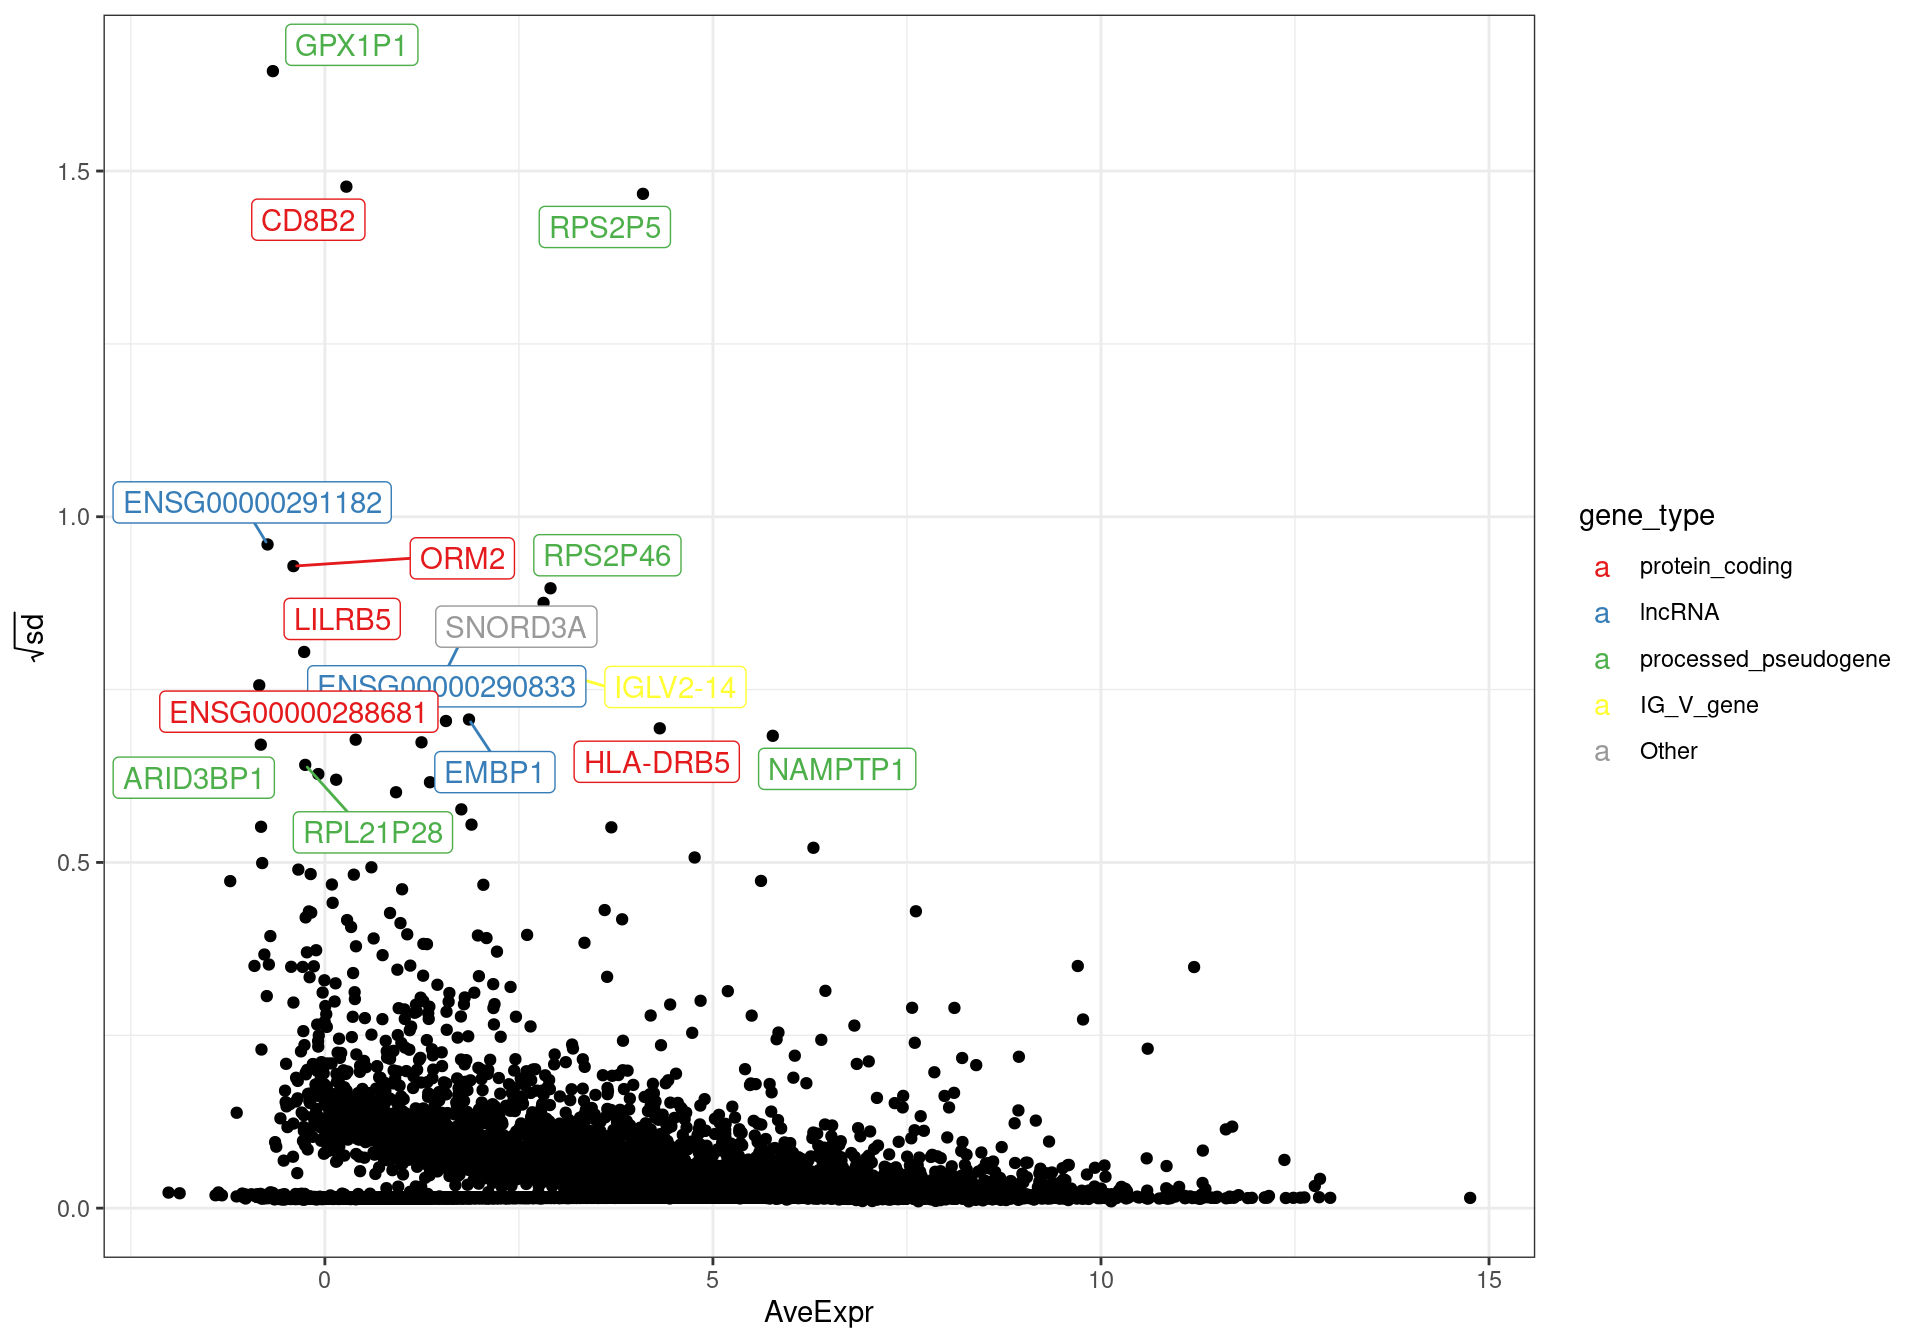
\includegraphics[scale=0.6]{sd-by-expr-1.png} 
			\textit{\normalsize Variability against average signal}\\[15mm]
		\end{minipage}

		\vspace{1cm}		
		\centering
		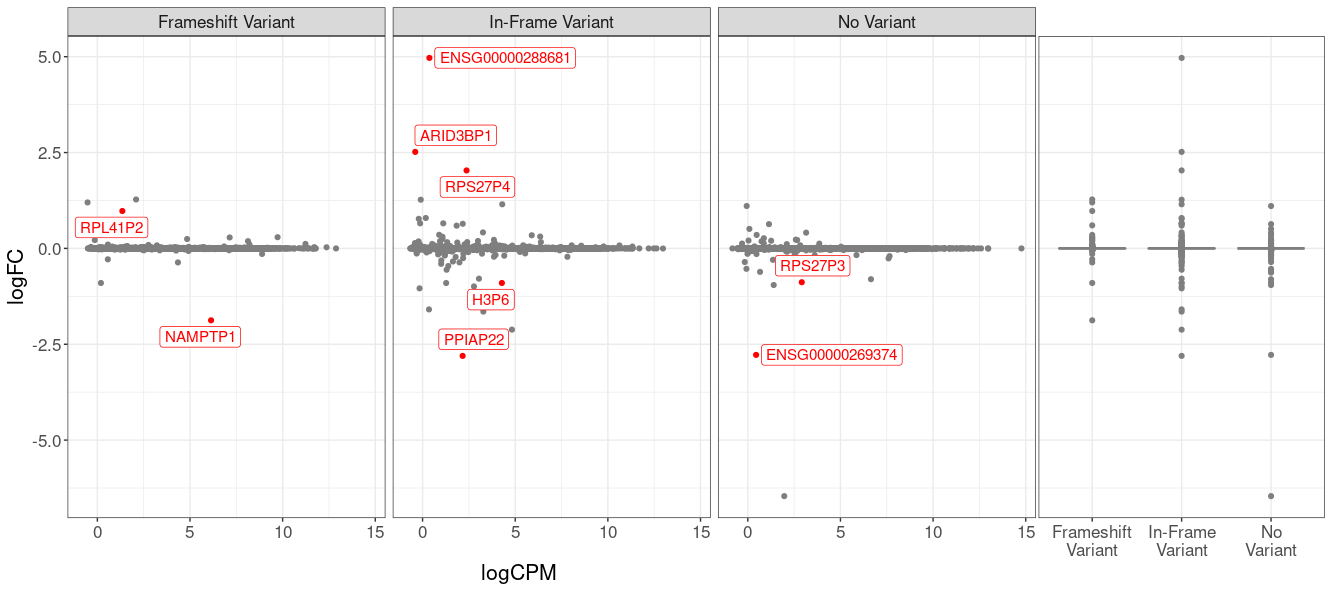
\includegraphics[scale=0.75]{ma-by-variant-1.png} 
		~\\
		\textit{\normalsize Differential Gene Expression results showing genes which passed an FDR of 0.05 for consideration as differentially expressed}\\[1cm]
		
	}
	
	\block{Developing a Variant-Modified Reference Transcriptome}{
	\large
	\begin{minipage}{0.2\linewidth}
		\centering
		
\includegraphics[scale=1]{transmogR.png}
	\end{minipage}
	\begin{minipage}{0.75\linewidth}
	\large
		The R package \texttt{transmogR}	has now been developed for using variants to modify a standard reference trancriptome, including decoy transcripts\autocite{Srivastava2020-tm}.
		This approach is coordinate-agnostic $\implies$ mapping back to regulatory features and GWAS results remains uncomplicated
	\end{minipage}		

	\vspace{1.5cm}
	

    \coloredbox{
	    \colorlet{innerblockbodybgcolor}{white}
        \innerblock{\large \textbf{References}}{
	        \printbibliography[heading=none]
		}
	 }
	    
   }


\end{columns}
\end{document}